\chapter{Word2vec -- Skipgram Approach}

\section{Vector embeddings and tokens}

    In these notes, we introduce a particular way to choose "good" vector embeddings, based on the word2vec technique.

    \begin{itemize}
        \item These notes were originally spliced from the Transformers chapter, so there are some regions of overlap.
    \end{itemize}


    \subsection{One-hot encoding isn't enough}

        First, we want to turn words into something computable, like a \gren{vector}.
            \note{It's difficult to try to do math on the word "cheddar". It's not numerical.}
    
        The simplest approach would be \vocab{one-hot encoding}.
            
        \begin{itemize}
            \item \miniex Suppose that we want to classify \textbf{furniture} as table, bed, couch, or chair.
        \end{itemize}
        
        \begin{equation}
            \begin{bmatrix}
              \text{table} \\ \text{bed} \\ \text{couch} \\ \text{chair} 
            \end{bmatrix}
        \end{equation}

        \begin{itemize}
            \item For each class:
        \end{itemize}
        
        
        \begin{equation}
            v_{chair} = 
            \begin{bmatrix}
              0\\0\\0\\ \red{1}
            \end{bmatrix}
            \qquad
            v_{table} = 
            \begin{bmatrix}
              \red{1}\\0\\0\\0
            \end{bmatrix}
            \qquad
            v_{couch} = 
            \begin{bmatrix}
              0\\0\\\red{1}\\0
            \end{bmatrix}
            \qquad
            v_{bed} = 
            \begin{bmatrix}
              0\\\red{1}\\0\\0
            \end{bmatrix}
        \end{equation}

        This approach is simple, but often, it's \textit{too} simple.\\

        \begin{concept}
            \vocab{One-hot encoding} loses a lot of information about the objects it's representing.

            \begin{itemize}
                \item It's hard to say which words are "\gren{similar}" to each other, for example.
            \end{itemize}
        \end{concept}

        \miniex You probably associate the word "\blu{sugar}" with "\blu{sweet}", and "\red{salt}" with "\red{savory}".

        \begin{itemize}
            \item But, if you use one-hot encoding, all of these words are "equally different".
                \note{You could \purp{shuffle} the rows of one-hot vectors, and represent the same information.
                
                \phantom{}
                
                So, we can't use the order of 1's and 0's to determine "closeness": the order can be \gren{freely changed}.}
        \end{itemize}

        \begin{equation}
            v_{salt} = 
            \begin{bmatrix}
              0\\0\\0\\ \red{1}
            \end{bmatrix}
            \qquad
            v_{savory} = 
            \begin{bmatrix}
              \red{1}\\0\\0\\0
            \end{bmatrix}
            \qquad
            v_{sugar} = 
            \begin{bmatrix}
              0\\0\\\red{1}\\0
            \end{bmatrix}
            \qquad
            v_{sweet} = 
            \begin{bmatrix}
              0\\\red{1}\\0\\0
            \end{bmatrix}
        \end{equation}

        In order to incorporate this information, we'll need a better way to represent words as vectors.

    \phantom{}

    \subsection{Word Embeddings: Similarity between words}

        Our new approach will convert each word $w$ into a \purp{vector $v_w$} of \gren{length $d$}.
            \note{Unlike one-hot encoding, we don't require that $d$ equals the size of our vocabulary.}

        \begin{equation}
            w \longrightarrow \pur{v_w} \qquad \qquad \pur{v_w} \in \grn{\RR^d}
        \end{equation}

        \textit{How} do we want to convert words into vectors? Above, we mentioned that one-hot doesn't tell us how \gren{similar} two words are.\\

        \begin{clarification}
            There are many ways for words to be \gren{similar}: similar word length, similar choice of letters, etc.

            But in our case, we're interested in \vocab{semantics}: the \purp{meanings} of the words. We want to know which words have similar meanings.
        \end{clarification}

        \begin{itemize}
            \item \miniex We don't consider "sugar" and "sweet" to be similar because they both start with "s". 
            
            \begin{itemize}
                \item They're similar because of \orgg{meaning}: sugar tastes sweet. Sweet strawberries contain sugar.\\
            \end{itemize}
        \end{itemize}

        \begin{concept}
            We often want our \vocab{word embeddings} $v_w$ to tell us which words are \gren{semantically similar} to each other: which words have similar \purp{meanings}.
            \begin{equation*}
                \text{$v_a$ and $v_b$ are \orgg{similar vectors}} 
                \;\;\iff\;\; 
                \text{$a$ and $b$ are \gren{semantically similar words}}
            \end{equation*}
        \end{concept}

        Our goal is to make this statement true. But we have a problem: these are \textit{concepts}, rather than computable \textit{numbers}. 

        \begin{itemize}
            \item So, we'll have to turn each side into something computable.
        \end{itemize}



    \phantom{}

    \subsection{Vector Similarity: Dot Products}

        First, we'll handle the left side: how do we know if vectors are \gren{similar}? 
        
        \begin{itemize}
            \item We've come across this problem multiple times, and we'll solve it the same way as always: using the \purp{dot product}.\\
        \end{itemize}

        \begin{concept}
            \textit{Review from the Classification chapter}
            
            You can use the \gren{dot product} between vectors $u$ and $v$, \purp{normalized by their magnitudes}, to measure their "\vocab{cosine similarity}". 

            \begin{equation*}
                S_C(u,v) = \frac{u \cdot v}{\abs{u} \cdot \abs{v}}
            \end{equation*}
            
            If two vectors are more \gren{similar}, they have a \gren{larger} normalized dot product. 

            \begin{itemize}
                \item This function ranges from -1 (opposite vectors) to +1 (identical vectors). Perpendicular vectors receive a 0.
            \end{itemize}
        \end{concept}

            \note{We call it "cosine similarity", because this is equal to the cosine of the angle $\alpha$ between $u$ and $v$.}

        \begin{figure}[H]
            \centering
            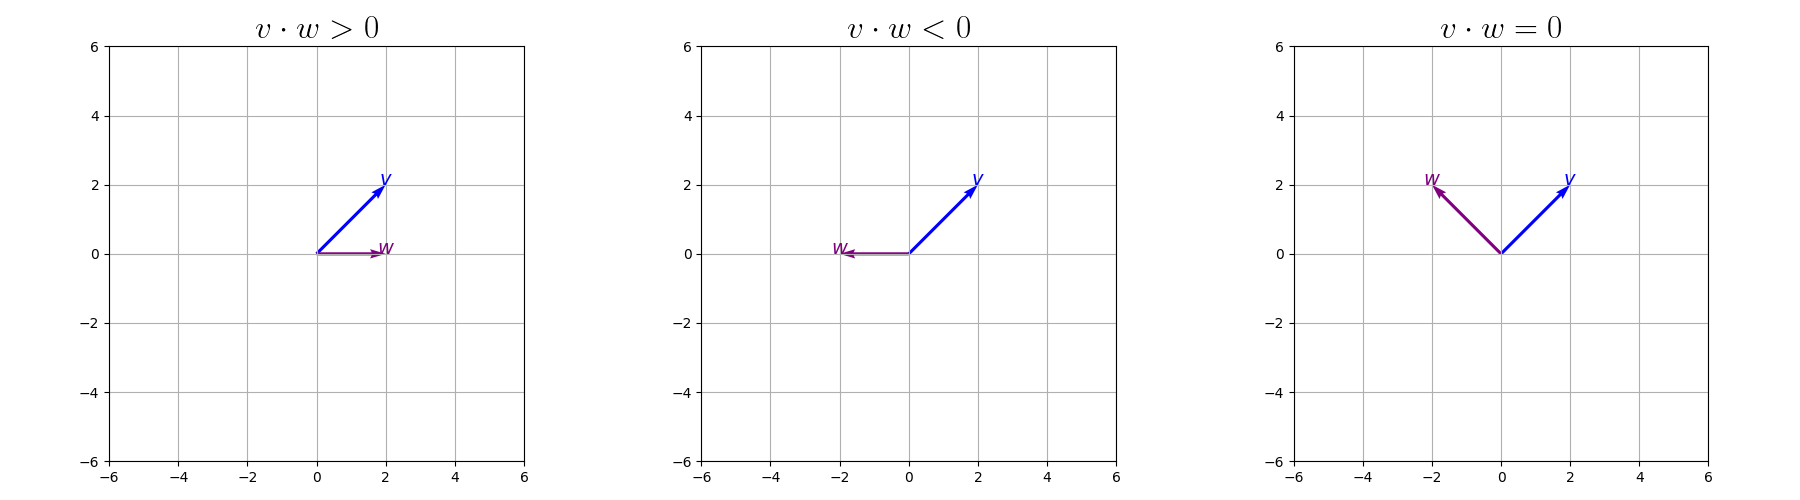
\includegraphics[width=140mm,scale=0.5]{images/transformers_images/dot_product_demo.png}
            
            
            \caption*{We can see here what we mean by "similar" or "dissimilar".}
        \end{figure}

        \begin{clarification}
            You can use $S_C(u,v)$ to measure the \gren{similarity} between two vectors, ignoring magnitude.

            But for simplicity, we'll skip the \purp{normalizing} step, and just take the \vocab{dot product}:

            \begin{equation*}
                S_D(u,v) = u \cdot v = u^\top v
            \end{equation*}
        \end{clarification}

        

        We're getting closer to a computable form:

        \begin{equation}
            \overbrace{ 
                (v_a \cdot v_b) \text{ is \orgg{large}}
            }^{\text{ \lblu{Similar vectors}}}
            \;\;\iff\;\; 
            \text{$a$ and $b$ are \gren{semantically similar words}}
        \end{equation}



    \phantom{}

    \subsection{Semantic Similarity and Word Frequency}

        The "right side" of our expression is a bit trickier: how do you compute which words have \gren{similar meanings}?

        We can't directly turn "meaning" into a number. But instead, we'll focus on a different concept, that might help us predict similarity:

        \begin{itemize}
            \item \miniex Earlier, we showed that "sweet and "sugar" were related, by referencing the fact that "\orgg{sugar tastes sweet}".

            \item While our machine might not understand the concept, it can see that "sugar" and "sweet" showed up \gren{together} in a sentence.
                \note{How much do/can large language models "understand" what they're saying? Lots of very smart people continue to argue exactly how much they know.}
        \end{itemize}

        Often, words that are related, show up in the same sentences, or paragraphs. So, we'll try to use this to our advantage:

        \begin{equation*}
            \text{$a$ and $b$ are \gren{semantically similar words}}
            \;\;\xLeftrightarrow{\text{maybe?}}\;\; 
            \text{$a$ and $b$ \purp{frequently} show up together}
        \end{equation*}

        These two aren't \textit{actually} equivalent, but we hope that we can use one to predict the other.\\

        \begin{concept}
            We can predict which words might be \orgg{more similar} by observing \purp{how often} they show up \gren{together} in a body ("corpora") of text.

            \begin{itemize}
                \item When two words occur \orgg{together} in a context, we call this \gren{co-occurrence}.
                \item Thus, we're measuring \vocab{frequency of co-occurrence}.
            \end{itemize}

            If two words show up near each other more frequently, we predict that they might be \gren{more similar}.

        \end{concept}

        This kind of word embedding is often called "\vocab{word2vec}", named after a particular set of algorithms that use this approach.
            \note{Sometimes, "word2vec" is used to reference any technology that creates word embeddings. But this isn't always technically accurate.}

        \begin{itemize}
            \item \miniex The words "quantum" and "physics" go together often. So do the words "rain" and "weather".\\
        \end{itemize}

        \begin{clarification}
            We \purp{don't actually know} for certain that, if two words often show up together, they have \orgg{related meanings}.

            But, in practice, we find that "\vocab{frequency of co-occurrence}" is a \gren{surprisingly good} measure of similarity.
        \end{clarification}

        Because we're talking about frequency, we'll consider the \gren{probability} of seeing both words together.

        \begin{equation*}
            \text{$a$ and $b$ are \gren{semantically similar words}}
            \;\;\xLeftrightarrow{\text{maybe?}}\;\; 
            \text{P \big( $a$ and $b$ \purp{occur together} \big) is \orgg{high}}
        \end{equation*}

        Finally, we have something closer to math:

        \begin{equation*}
            \overbrace{
                v_a \cdot v_b \text{ is \orgg{large}}}
            ^{\text{Similar vectors}}
            \;\;\iff\;\; 
            \overbrace{
                \text{P \big( $a$ and $b$ \purp{occur together} \big) is \orgg{high}}}
            ^{\text{Similar words}}
        \end{equation*}

        Now, we have some "mathematical" concepts: we can start using these to create mathematical \textbf{objects}.


    \phantom{}
    
    \subsection{Clarifying our probability}

        In order to proceed, we need to be a little more specific.

        \begin{equation*}
            \overbrace{
                (v_a \cdot v_b) \text{ is \orgg{large}}}
            ^{\text{Similar vectors}}
            \;\;\iff\;\; 
            \overbrace{
                \text{P \big( $a$ and $b$ \purp{occur together} \big) is \orgg{high}}}
            ^{\text{Similar words}}
        \end{equation*}

        
        The dot product is already an equation, so the left side is fine.

        \phantom{}
        
        The right side is all we need to clear up: "P \big( $a$ and $b$ \purp{occur together} \big)" is a bit \gren{vague}. 
            \note{One interpretation would be: "if we look at a random phrase, how often do we have words $a$ and $b$?"

            \phantom{}
            
            But we only care whether $a$ and $b$ are together/separate: we don't care about sentences containing neither.}
        
        \begin{itemize}
            \item We want to know if $a$ and $b$ tend to show up \orgg{together}, rather than \purp{separately}.
        \end{itemize}

        Here's a concrete way to say this: "\gren{if} we find one word, \purp{how often} do we find the other nearby?"\\

        \begin{concept}
            To predict how \gren{similar} words $a$ and $b$ are, we want to compute how often they \vocab{co-occur}.

            \begin{itemize}
                \item One way to phrase this: "\gren{given} that we find $a$, what are the \purp{chances} we find $b$ nearby?"
            \end{itemize}

            \begin{equation*}
                \given{b \text{ nearby} }{a \text{ found}}
            \end{equation*}
        
        \end{concept}

        \begin{equation*}
            \overbrace{ 
                (v_a \cdot v_b) \text{ is \orgg{large}}
            }^{\text{ \lblu{Similar vectors}}}
            \;\;\iff\;\; 
            \overbrace{
                \text{ $\given{b \text{ nearby} }{a \text{ found}}$  is \orgg{large}}}
            ^{\text{\lblu{Occur together frequently}}}
        \end{equation*}

        We're getting warmer! 
        
        \begin{itemize}
            \item We "\purp{find}" $a$ at index $t$: 
                \note{$w_t$ is the $\nth{t}$ word in our passage.}

                \begin{equation}
                    w_t=a
                \end{equation}

            \item Now, let's define what it means for $b$ to be "\gren{nearby}".\\
        \end{itemize}


        \begin{definition}
            In a text, we may want to find the "context" for \gren{center word} $w_t$: we want all of the words \orgg{nearby}.

            \begin{itemize}
                \item We'll use the $c$ nearest words on either side: these are our \purp{context words}. $c$ is our \vocab{maximum skip distance}.
            \end{itemize}

            This collection of $2c+1$ words is called our \vocab{context window}.

            \begin{equation*}
                \begin{matrix}
                    \cdots & w_{t-4} & 
                    \overbrace{
                    \begin{matrix}
                        \pur{w_{t-3}} & \pur{w_{t-2}} & \pur{w_{t-1}} &
                        \grn{w_t} & 
                        \pur{w_{t+1}} & \pur{w_{t+2}} & \pur{w_{t+3}}
                    \end{matrix} 
                    }^{\text{  Context window for $c=3$}}
                    & w_{t+4} & \cdots
                \end{matrix}
            \end{equation*}
            
        \end{definition}

            \note{We call $c$ our "maximum skip distance", because it's the largest number of words we can "skip" over, starting from $w_t$. 
            
            \phantom{}
            
            We're allow to move over by $c$ words, in either direction.}

        \begin{itemize}
            \item Notice the similarity to the filter size from Convolution: we still have an idea of "locality".
        \end{itemize}


        \phantom{}

        So, we want to look for $b$ in our context window. There are two ways we can turn this into a probability:

        \begin{itemize}
            \item You check all of the context words \orgg{at the same time}:

            \begin{equation}
                \begin{matrix}
                    \cdots & w_{t-3} & 
                    \overbrace{
                    \begin{matrix}
                        \pur{w_{t-2}} & \pur{w_{t-1}} & \grn{w_t} & \pur{w_{t+1}} & \pur{w_{t+2}}
                    \end{matrix} 
                    }^{\text{ All words within $c=2$ context window}}
                    & w_{t+3} & \cdots
                \end{matrix}
            \end{equation}

            \item You check \gren{one word at a time}: $j$ units to the right/left.

            \begin{equation}
                \begin{matrix}
                    \cdots & w_{t-3} & 
                    \overbrace{
                    \begin{matrix}
                        \blu{w_{t-2}} & w_{t-1} & \red{w_t} 
                    \end{matrix} 
                    }^{\text{Only $w_{t-2}$. Thus, $j=-2$}}
                    & w_{t+1} & w_{t+2}
                    & w_{t+3} & \cdots
                \end{matrix}
            \end{equation}
        \end{itemize}

        For now, it's easier to use the latter approach: \gren{each index} has a \purp{separate probability}.\\

        \begin{concept}

            We measure the \vocab{co-occurrence} of $a$ and $b$ by asking:

            \begin{itemize}
                \item "\orgg{Given} that we find $a$ at index $t$...

                \begin{equation*}
                    \grn{w_t=a}
                \end{equation*}
                
                \item what are the \orgg{chances} that we find $b$ at index $t+j$?"
                
                \begin{equation*}
                    \pur{w_{t+j} = b}
                \end{equation*}
            \end{itemize}

            With this, we find our result:

            \begin{equation*}
                \given{ \pur{w_{t+j} = b} }{ \grn{w_t=a} }
            \end{equation*}
            
        \end{concept}

        We did it! This is a clear, explicit probability.

        \begin{equation*}
            \overbrace{ 
                (v_a \cdot v_b) \text{ is \orgg{large}}
            }^{\text{ \lblu{Similar vectors}}}
            \;\;\iff\;\; 
            \overbrace{
                \given{ \pur{w_{t+j} = b} }{ \grn{w_t=a} } \text{ \quad is \orgg{large}}}
            ^{\text{\lblu{Occur together frequently}}}
        \end{equation*}

        \begin{notation}
            We can make this notation a little denser: 

            \begin{equation*}
                \given{ \pur{w_{t+j} = b} }{ \grn{w_t=a} }
                \quad=\quad
                \given{ b }{ a }_j
            \end{equation*}

            This assumes that $t$ \redd{doesn't} affect our probability: it doesn't matter \gren{where} we found $a$, just \purp{how far away} $b$ is (and on which side).

            \begin{itemize}
                \item This is a reasonable assumption for our purposes.
            \end{itemize}
        \end{notation}




    \phantom{}

    \subsection{Computing predicted probabilities}

        How do we turn a \gren{real number} $v_a \cdot v_b$ into a \purp{probability} $P\big(b \; | \; a\big)_j$? 

        \begin{itemize}
            \item $P\big(b \; | \; a\big)_j$ is the chance of finding $b$ at index $t+j$, if $a$ is at index $t$.

            \begin{equation}
                \begin{matrix}
                    \cdots & w_{t-3} & 
                    \overbrace{
                    \begin{matrix}
                        \blu{w_{t-2}} & w_{t-1} & \red{w_t} 
                    \end{matrix} 
                    }^{\text{What word is at $w_{t-2}$? Is it $b$?}}
                    & w_{t+1} & w_{t+2}
                    & w_{t+3} & \cdots
                \end{matrix}
            \end{equation}
            \item So, we need to compare $b$ to every other word that we could find at $t+j$: this is a \orgg{multi-class problem}, using the \vocab{softmax function}.
                \note{We have one class for each possible word we could find at $t+j$.}
        \end{itemize}

        \begin{equation}
            \operatorname{Softmax}(z_k) = \frac{e^{z_k}}{ \sum_i e^{z_i}}
        \end{equation}

        Let's review the concept behind "softmax":\\

        \begin{concept}
            Suppose that we have \purp{$n$ possible words} ($n$ "classes"), and we want to figure out which one is \gren{correct}.
            
            The \vocab{$\nth{k}$ class} has a score, \org{$z_k$}, used to compute probability.

            \begin{itemize}
                \item The bigger $z_k$ is, the \purp{more likely} $k$ is to be the \gren{correct class}.
            \end{itemize}

            \phantom{}

            To keep it \gren{positive}, $z_k$ is converted to \org{$e^{z_k}$}: each $e^{z_i}$ competes to see which class is more likely.

            \begin{itemize}
                \item To create a probability, we \purp{compare} the score of class $k$ to all of our other classes, using \vocab{softmax}.
            \end{itemize}

            \begin{equation*}
                \overbrace{
                    e^{z_k}}^{\text{\lblu{Class k}}} 
                \text{\; vs \;} 
                \overbrace{ 
                    \sum_i e^{z_i} }^{\text{\lblu{All classes}}}
                \quad \quad \Longrightarrow \quad \quad  \operatorname{Softmax}(z_k) = \frac{e^{z_k}}{ \sum_i e^{z_i}}
            \end{equation*}
            
        \end{concept}

        \begin{itemize}
            \item We repeat this process for every possible word $i$, to get all of our predictions.
        \end{itemize}

        Now, the big question: what is $z_k$?

        \begin{equation*}
            \overbrace{ 
                (v_a \cdot v_b) \text{ is \orgg{large}}
            }^{\text{ \lblu{Similar vectors}}}
            \;\;\iff\;\; 
            \overbrace{
                \given{ \pur{w_{t+j} = b} }{ \grn{w_t=a} } \text{ \quad is \orgg{large}}}
            ^{\text{\lblu{Occur together frequently}}}
        \end{equation*}

        $z_k$ and $(v_a \cdot v_b)$ serve the \vocab{same purpose}:

        \begin{itemize}
            \item Large \gren{dot product} predicts high probability.
            \item Large \pur{$z_k$} predicts high probability.
        \end{itemize}

        So, we can use our dot product as a "score" $z_k$:

        \begin{equation}
            z_b = \red{v_a} \cdot \grn{v_b}
        \end{equation}

        Now, we can plug this into our probability equation!\\

        \begin{kequation}
            The \gren{more similar} (bigger dot product) $a$ and $b$ are, the \purp{more likely} we predict to find them together.

            \begin{itemize}
                \item We use a \vocab{softmax} to compute this probability for each possible word $b$.
            \end{itemize}

            \begin{equation*}
                    \given{ \grn{w_{t+j} = b} }{ \red{w_t=a} } 
                    \quad=\quad
                    \frac{e^{\red{v_a} \cdot \grn{v_b}} }{ \sum_i e^{\red{v_a} \cdot \blu{v_i} }}
            \end{equation*}

            Or, in alternate notation: 
            
            \begin{equation*}
                \given{ \grn{b} }{ \red{a} } 
                \quad=\quad
                \frac{  \phantom{ \Bigg|} 
                \exp \Big(\red{v_a} \cdot \grn{v_b}\Big) }
                {\phantom{ \Bigg|}
                \sum_{\blu{i}} \exp \Big(\red{v_a} \cdot \blu{v_i} \Big) }
            \end{equation*}
        \end{kequation}

        Ta-da! We've combined two separate concepts into a single equation.
            \note{Note that, in both top and bottom, we keep \red{$v_a$}: we're considering every possible word for \blu{$w_{t+j}$}, while we \textit{know} \red{$w_t=a$}.}



    \phantom{}

    \subsection{Skip-gram approach: Training our word2vec model}

        One remaining issue: this equation doesn't tell us what the "true" probabilities are: they tell us the probability that our model \purp{predicts}.
        
        \begin{itemize}
            \item Now, we have to choose a \gren{good model} (word embedding).\\
        \end{itemize}
        
        \begin{clarification}
            Our equation is $\given{ \grn{w_{t+j} = b} }{ \red{w_t=a} }$ is our \orgg{estimation} for the probability.

            \begin{itemize}
                \item The real probabilities could be \purp{different}: we'll design our word embedding to give us the most \gren{accurate probabilities}.
            \end{itemize}
        \end{clarification}

        First: what does our model look like? How do we even \orgg{generate} word embeddings?

        \begin{itemize}
            \item Often, we rely on a neural network.\\
        \end{itemize}

        \begin{definition}
           We have two common \vocab{models for word embedding} ($\theta$):

            \begin{itemize}
                \item Separately assigning a \gren{vector} to each word.
                \item Using a shared \purp{neural network} to embed every word as a vector.
            \end{itemize}

            Our neural network uses \gren{parameters} $\theta$. We'll use $\theta$ to represent our embedding, that we want to \orgg{train}.

            \begin{equation*}
                \grn{w} \xlongrightarrow{\theta} v_{\grn{w}}
            \end{equation*}
        \end{definition}

        How do we pick a good model? 

        \begin{itemize}
            \item We'll \gren{train} our embedding $\theta$, so that our \purp{probabilities} are as accurate as possible.
        \end{itemize}

        As we established, our problem is multi-class classification:\\

        \begin{concept}
            \textit{Review from Classification chapter}

            For \vocab{multi-class classification}, we use the \gren{negative log-likelihood multiclass} (NLLM) equation to compute \purp{loss}:

            \begin{equation*}
                \loss_{NLLM}
                (\red{g} , \blu{y})
                =
                -\sum_{i=1}^n
                y_i \log(g_i)
            \end{equation*}

            $y$ is a one-hot vector, so all terms of the sum except the "correct" term $i=k$ cancel out to 0:

            \begin{equation*}
                -\blu{y_k} \log(\red{g_k})
                \qquad \xlongrightarrow{y_k=1  } \qquad
                -\log(\red{g_k})
            \end{equation*}
        \end{concept}

        $g_k$ is the probability we assigned to the correct answer.

        Next, we need training data: a body of \purp{text}.

        \begin{itemize}
            \item For an example, let's visit index $t$ in the text: this is the center of our \vocab{context window}. 
            \item $a$ is replaced by whatever word we find at that index: \red{$w_t$}. We still want to predict \blu{$w_{t+j}$}.
        \end{itemize}

        \begin{equation}
            \begin{matrix}
                \cdots & w_{t-3} & 
                \begin{matrix}
                    w_{t-2} & w_{t-1} & \red{w_t} 
                \end{matrix} 
                & \cdots & \blu{w_{t+j}}
                & w_{t+j+1} & \cdots
            \end{matrix}
        \end{equation}

        How good is our word embedding? According to NLLM: "how likely were we to correctly predict $w_{t+j}$?"

        \begin{equation*}
            \loss_{NLLM}(\red{g},\blu{y}) = -\log \Big(
                \given{\text{\grn{Correct word for index $t+j$}}}{\red{w_t}} 
            \Big) 
        \end{equation*}

        The correct word for index $t+j$ would be... $w_{t+j}$. We can read the outcome from the text, and use our model to check how \purp{likely} we thought that outcome was.

        \begin{equation*}
            \loss_{NLLM}(\red{g},\blu{y}) = -\log \Big(
                \overbrace{
                \given{\grn{w_{t+j}}}{\red{w_t}} 
                }^{\text{How likely we thought $w_{t+j}$ was, based on model}}
            \Big) 
        \end{equation*}

        Note that, the higher this probability is (the more sure we are of the correct answer), the closer the loss gets to 0.\\

        \begin{kequation}
            We train our \vocab{word embedding} $\theta$ by \purp{maximizing} the probability $\mathbf{P}(\grn{w_{t+j}} \quad|\quad \red{w_t})$ of predicting the \gren{correct word} in each spot.

            In our case, we want to \purp{minimize}

            \begin{equation*}
                \loss_{NLLM}(\theta,j) = -\log \Big(
                    \given{\grn{w_{t+j}}}{\red{w_t}} 
                \Big) 
            \end{equation*}
            where

            \begin{equation*}
                \given{ \grn{b} }{ \red{a} } 
                \quad=\quad
                \frac{  \phantom{ \Bigg|} 
                \exp \Big(\red{v_a} \cdot \grn{v_b}\Big) }
                {\phantom{ \Bigg|}
                \sum_{\blu{i}} \exp \Big(\red{v_a} \cdot \blu{v_i} \Big) }
            \end{equation*}
        \end{kequation}

        Now, we know how to compute these odds for a \purp{single index}, $t+j$. We want to repeat this process for the rest of our context window:


        \begin{equation}
            \begin{matrix}
                \cdots & w_{t-3} & 
                \overbrace{
                \begin{matrix}
                    \pur{w_{t-2}} & \pur{w_{t-1}} & \grn{w_t} & \pur{w_{t+1}} & \pur{w_{t+2}}
                \end{matrix} 
                }^{\text{ All words within $c=2$ context window}}
                & w_{t+3} & \cdots
            \end{matrix}
        \end{equation}

        \begin{kequation}
            We can find the \purp{total loss} of our embedding $\theta$, over our entire \vocab{context window}, by adding up the loss from each \gren{context word}.
            
            This includes all of the indices $(t+j)$, going from $j=-c$ to $j=+c$. Meaning, we want 

            \begin{itemize}
                \item \org{$|j| \leq c$} (within window) 
                \item \pur{$j \neq 0$} (don't want to compare $w_t$ with itself)
            \end{itemize}

            

            \begin{equation*}
                \loss_{t}(\theta) = - \sum_{\org{|j| \leq c}}^{\pur{j \neq 0}}
                \log \Big(
                    \given{\grn{w_{t+j}}}{\red{w_t}} 
                \Big) 
            \end{equation*}
        \end{kequation}

        One more modification: the loss function above only computes loss for a \gren{single context window}.

        But, for a passage of text, there are many possible context windows: all we have to do is shift our target word, $w_t$.

        \begin{itemize}
            \item \miniex Below, with $c=2$, we'll show all of our possible context windows: 
                \note{Target word is red, context words are blue.}
        \end{itemize}

        \begin{equation}
            \begin{matrix}
                \text{\red{This} \blu{is a} sample sentence} \\
                \text{\blu{This} \red{is} \blu{a sample} sentence} \\
                \text{\blu{This is} \red{a} \blu{sample sentence}} \\
                \text{This \blu{is a} \red{sample} \blu{sentence}} \\
                \text{This is \blu{a sample} \red{sentence}} 
            \end{matrix}
        \end{equation}

        We'll average the loss over \orgg{all context windows}.
            \note{We'll ignore negative indices, so we don't cause problems when $t=0$ or $t=T$.}\\

        \begin{kequation}
            Take a body of text with $T$ words, and a \purp{context window} with a \gren{max skip distance} of $c$. We use word embedding $\theta$.

            Our \orgg{objective function} $J(\theta)$ for the \vocab{skip-gram word2vec} algorithm, over the entire passage, is:

            \begin{equation*}
                J(\theta) = \frac{1}{T} \sum_{t=1}^T \loss_{t}(\theta)
            \end{equation*}

            or,

            \begin{equation*}
                J(\theta) = -\frac{1}{T} \sum_{t=1}^T 
                \quad
                \Bigg( \quad
                    \sum_{\org{|j| \leq c}}^{\pur{j \neq 0}}
                    \log \Big(
                        \given{\grn{w_{t+j}}}{\red{w_t}} 
                    \Big) \quad
                \Bigg)
            \end{equation*}
        \end{kequation}

            

        This is the completed loss function that we can use to train our embedding.\\

        \begin{concept}
            We can train our \gren{embedding} $\theta$ using our \purp{loss function} $J$, via \vocab{gradient descent}.

            \begin{equation*}
                \grn{\theta'} = \grn{\theta} - \eta \nabla_{\grn{\theta}}\pur{J}
            \end{equation*}

            \begin{itemize}
                \item If we're using a \orgg{neural network} to create embeddings, we'll need \phantom{fillertonextline} \vocab{back-propagation} to train.
            \end{itemize}
        \end{concept}




    \pagebreak




    \subsection{Issues with skip-gram}

        There are a few problems worth addressing. First, look again at our equation:

        \begin{equation*}
                \given{ \grn{w_{t+j} = b} }{ \red{w_t=a} } 
                \quad=\quad
                \frac{e^{\red{v_a} \cdot \grn{v_b}} }{ \sum_i e^{\red{v_a} \cdot \blu{v_i} }}
        \end{equation*}

        Something might strike you: our probability is \purp{totally independent} of which index $t+j$ we want to predict.

        \begin{itemize}
            \item That means, our model would make the exact same prediction for every nearby word.
            \item This is more easily resolved in our transformer model, so we won't worry about it for now.\\
        \end{itemize}

        \begin{concept}
            Our \purp{probability} calculation in skip-gram is \gren{independent} of the \vocab{skip distance} $j$ between words $w_t$ and $w_{t+j}$.

            \begin{itemize}
                \item All words within the \vocab{context window} have the \orgg{same probability distribution}.
            \end{itemize}
        \end{concept}


        Another problem: if "more \gren{similar}" means "more likely to \orgg{co-occur}", doesn't that suggest that we would expect a word to appear with itself, really often?

        \begin{itemize}
            \item This would be true for every word: nothing can be more similar to a vector than itself, after all.

            \item Our solution is to just \purp{exclude} $w_t$ from predictions about nearby words.\\
        \end{itemize}

        \begin{concept}
            The most similar word to $w_t$, is \orgg{itself}!

            \begin{itemize}
                \item So, we often \purp{exclude} $w_t$ from predictions.
            \end{itemize}
        \end{concept}


        Another problem: our objective function $J(\theta)$ includes a logarithm. To optimize $\theta$, we'd need to compute its \purp{derivative}.

        \begin{itemize}
            \item This becomes really expensive, especially when our vocabulary can have millions of words.

            \item Our solution is to "\orgg{prune}"/remove a lot of words from our probability calculation.
                \note{We can predict in advance, that some words don't need to be included.}\\
        \end{itemize}
            
        \begin{concept}
            \vocab{Skip-gram} can become expensive to train, when the \gren{vocabulary} becomes too large.

            \begin{itemize}
                \item So, we \orgg{prune} some unlikely words in our vocabulary, to speed up our \purp{predictions}.
            \end{itemize}
        \end{concept}